\documentclass[11pt]{article}
\usepackage[utf8]{inputenc}
\usepackage{geometry}
\geometry{a4paper, portrait, margin=2cm}
\usepackage[english]{babel} 
\usepackage{parskip}
\usepackage{chngcntr}
\counterwithin{figure}{section}
\usepackage{url}
\usepackage[noadjust]{cite}
\usepackage{mathtools}
\usepackage[nottoc,numbib]{tocbibind}
\usepackage{graphicx}
\usepackage{pdflscape, lscape}
\usepackage{array}
\usepackage{gensymb}
\usepackage{tabularx}
\usepackage{caption}
\usepackage{everypage}
\usepackage{amsmath}
\usepackage{mathtools}
\usepackage{enumitem}
\setlist{noitemsep}

\title{An Evaluation of Cooperative Handheld Robotics in a Simplified 3D Construction Environment}
\author{Chris Meehan}

\begin{document}

\begin{titlepage}
	\centering
	
	
\includegraphics[width=0.6\textwidth]{bristol.png}
	\vspace{2cm}

	{\huge\bfseries The Design and Evaluation of a Four Degree-Of-Freedom Cooperative Handheld Robotic Device in a Simplified 3D Construction Environment\par}
	\vspace{1.5cm}

	{\Large\itshape By Chris Meehan\par}
	
	Supervised by\par
	Dr. Walterio Mayol-Cuevas
	
	\vspace{1.5cm}
	
	Department of Computer Science\par
	University of Bristol

	\vfill

% Bottom of the page
	{\large \today\par}
\end{titlepage}

\section{Executive Summary}
\pagebreak

\section{Acknowledgements}
\pagebreak


\tableofcontents
\pagebreak

\section{Introduction}
\pagebreak

\section{Aims and Objectives}
\pagebreak

\section{Research Review}
\subsection{Robotics with Humans In-The-Loop} \label{intheloop}

Although robots have become vastly more capable over recent years with technological improvements, many tasks still require some form of human assistance in order for the objectives to be adequately met. Robots can be perfectly equipped to handle operations which involve precise motion or repetitive tasks, which may be present physical challenges to humans \cite{Chipalkatty2012}. Conversely, they still lack ability in areas which require the high-level cognitive reasoning that comes naturally to humans. As such, there exists many applications in which humans are in-the-loop for robotic operations. This applies to both forms of robotics that the handheld area sits between; external robots and, especially so, wearable technology.  

\subsubsection{Safety}

Perhaps the most important factor in these situations is how the robot receives and processes user intent. An input from the user should be analysed by the robot in terms of importance and the choice of subsequent actions should be made appropriately. A prime example of where this is of paramount concern is in vehicular operations, where potential accidents could be catastrophic. Anderson et al \cite{Anderson2010} investigated a semi-autonomous hazard avoidance framework and tested it in a real-life driving environment, where the human driver received full control during non-threat situations. However, in times of threat detection, the control system became fully autonomous and guided the car to the safety. In this situation, the robot assumed the expertise of hazard assessment and reaction time, whereas the human provided general navigation that was accepted by the system under normal circumstances. This is one extreme, where the human input is essentially ignored under certain conditions for the safety of the user and those nearby. 

The other end of the spectrum, human input must be immediately responded to in order to act safely, where it is assumed the human possesses greater threat detection. Thus safety to both the human and robot must be positively ensured \cite{Haddadin2007}. In industrial applications, the robot often operates in an isolated workspace from the human, where an extreme human input would constitute an emergency button or entering the workspace via a safety door/light gate, which the robot must respond to by halting all physical actions for human safety \cite{ISOGuards}. However, it is growing increasingly common for the robot and human to share the same workspace, occasionally cooperating in a physical manner, such as the humanoid robot presented by Ott et al \cite{Ott2006} and illustrated in Figure \ref{figure:humanoid}.

\begin{center}
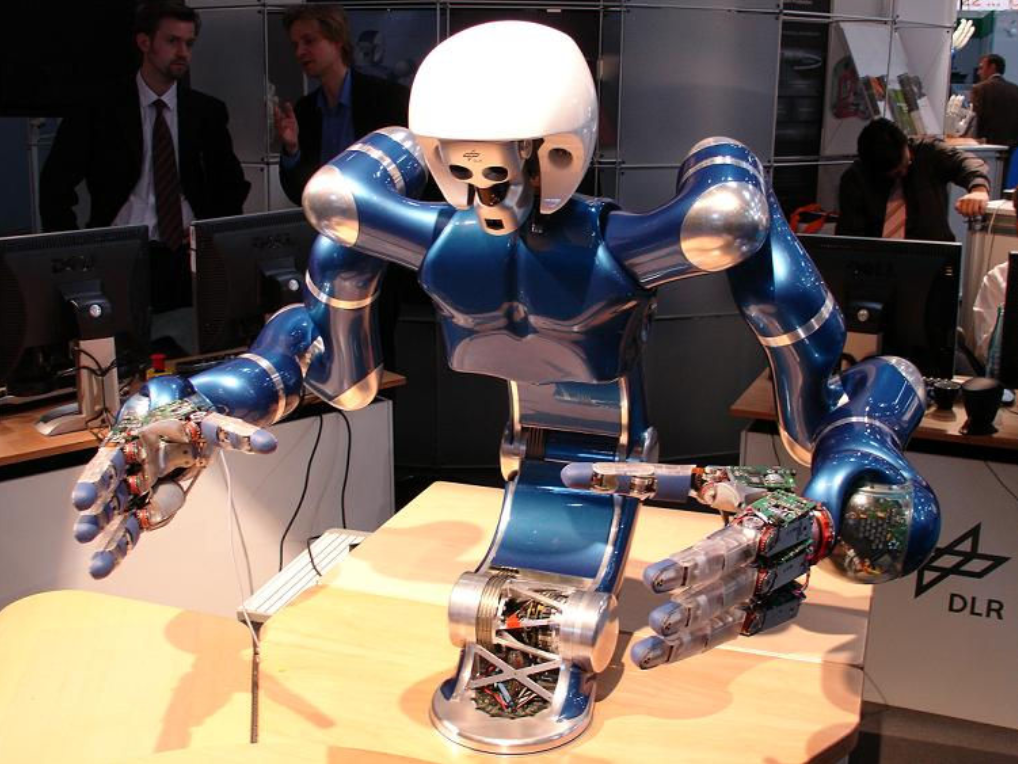
\includegraphics[width=0.48\textwidth]{humanoid.png}
\captionof{figure}{Two-Arm Humanoid for Dexterous Manipulation, image from \cite{Ott2006}.}
\label{figure:humanoid}
\end{center}

Existing operational requirements for collaborative robots have been specified in IS0-10218, which focus on defining the upper limit of either the tool centre point velocity, the dynamic power, or the static force. However, as discussed by Haddadin et al \cite{Haddadin2007}, these values are merely based on heuristics. As such, more specific severity indices were introduced, taking from biomechanically motivated quantities.

\subsubsection{Autonomy Study}
The reliability offered by human controllers can rarely be matched by autonomous agents. Similarly, the efficiency afforded by robots is highly attractive in physical tasks. Finding a strong balance between the two is essential in successfully accomplishing a task. Heger et al \cite{heger2006} investigate a mode of shared control, referred to as ``Sliding Autonomy". Fundamentally, this is an analysis to find the optimal flow of control between autonomous agents and a human operator for a given task, where an operator observes the operation and intervenes when necessary. A scenario was performed based on the model where three robots work cooperatively with a human operator to assemble a physical structure, with numerous failure modes deliberately implemented. The results indicated that the cooperation compromise resulted in task efficiency similar to a fully autonomous mode, while maintaining a level of reliability associated with teleoperation systems (remote human control). The constant attention of the human, without being cognitively demanding, improved the success rate while acting as a safety net for failures that the robot alone cannot recover from.

There are plenty of other investigations into the study of variable autonomy, such as in \cite{Dorais1999}, which looks into variable interactions in space missions, and in \cite{tambe2002}, which concentrates on the costs (time delays and other effects) of such transfer-of-control systems. Although this area of interchangeable control is mostly focused on with regard to external robotics, it is still relevant to the handheld field. As covered in \cite{GreggSmithDesign}, examining the varying degrees of autonomy that a handheld robot may exhibit for a given task is necessary to locate the control set-up to give optimal performance.
A different approach was taken to shared control in \cite{Poncela2009}, where the efficiency offered by both members in the cooperation was measured at each time instant from the point of view of reactive strategy. The experiment in this paper focused on the shared navigation of a Pioneer AT robot, where the commands of both the human and the robot were weighted and linearly combined, resulting in a single motory operation, as illustrated in Figure \ref{figure:autocar}.

\begin{center}
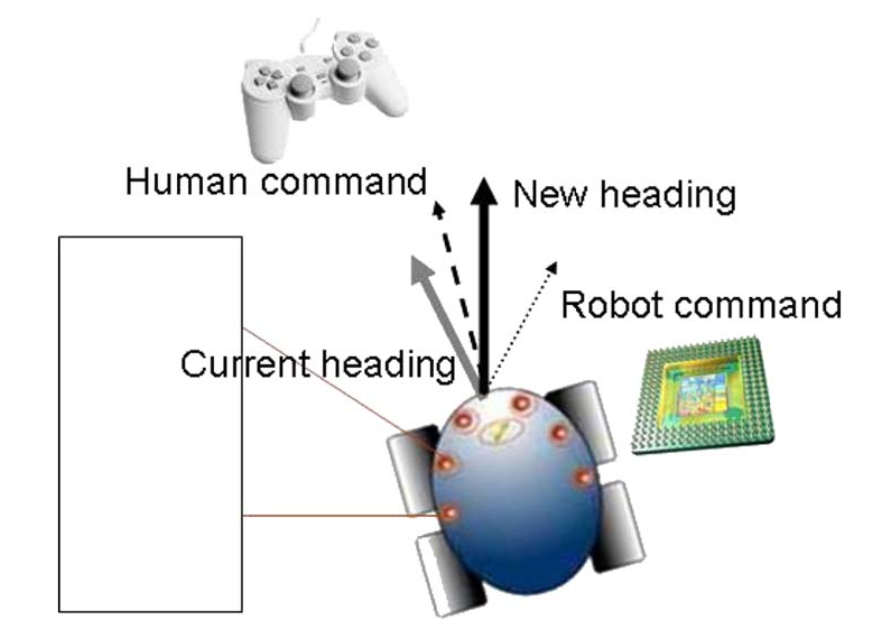
\includegraphics[width=0.48\textwidth]{autocar.png}
\captionof{figure}{Resulting command from human and robot inputs, image from \cite{Poncela2009}.}
\label{figure:autocar}
\end{center}

The results of this experiment showed that the weighting between the two inputs led to performance which did not match that offered by each member alone, but did seem to combine the benefits of both when taking a range of scenarios into consideration. This is a rare situation in which the task at hand could be performed with equal skill by both human and robot, and caters to the speciality of neither. However, the approach of taking a weighting between the two inputs is interesting. It may be worth investigating such a method with the handheld robot in the future. This would entail combining the two signals and deciding the action based on the weighting the given scenario. In such a case, a range of different settings could be explored, as opposed to just three discreet levels of autonomy as was the case in \cite{GreggSmithDesign}. However, such an investigation would require a large number of participants, performing tasks with a large variety of weightings. This is outside the scope of the current project.

\subsubsection{Collaboration with Assistive Robotics}
Rather than replacing human operations, robotics can be employed to assist in them, maintaining human flexibility while increasing productivity. One such case where this is applicable is in the manufacturing industry, particularly assembly. Robots with highly specific purposes have long been used on assembly lines to increase output, performing simple and repetitive tasks at a faster rate than is possible with human workers. However, humans are frequently used for more complicated procedures that require motion in multiple degrees of freedom. The adaptability and range of motion of human workers is often unrivalled compared with traditional robotics, as well as being much more available. 

A sensible compromise is investigated in \cite{lenz2011}, where robotics are used to provide assistance to a human-oriented assembly task. A Hidden Markov Model (HMM) based analysis was used so that the robot may predict the next stages of the task, lending assistance by passing the required components to the user at the appropriate time so that they may continue with the operation. As a pre-requisite for any useful interaction between the human and the robot, the robot must first be trained. In order to accomplish this, the assembly tasks were performed solely by the human whilst sensors were used at various hand and body positions, so that the task motions could be adequately tracked. A similar study, focused primarily on the timing of assistance, contains an in-depth description of this preliminary set-up \cite{huber2010}. The task comprised the assembly of a six-block tower, bolting the blocks together in varying manners. Once the data was collected for the human performed task with sensors, the results were used to form the model.

The model generated in \cite{lenz2011} could then be transferred to the robotic platform JAHIR (Joint-Action for Humans and Industrial Robots). This hybrid assembly platform for the context outlined in the paper is illustrated in Figure \ref{figure:jahir}. Both the robot and the human share a designated workspace, whereas the storage areas for the parts are only accessible by the robot. An interaction area exists which overlaps with the human workspace, in which the robot may assist by transporting required parts to within human reach. There are numerous options for estimating the progress of human-performed tasks, one such technique is the one used for the preliminary experiment; strategically placed accelerometers and microphones. This technique is outlined in detail in \cite{lukowicz2004}, where most workshop activities could be identified at 84.4\% accuracy. In the case of the preliminary experiment in \cite{lenz2011}, pertaining solely to the assembly task, greater accuracies were achieved.

\begin{center}
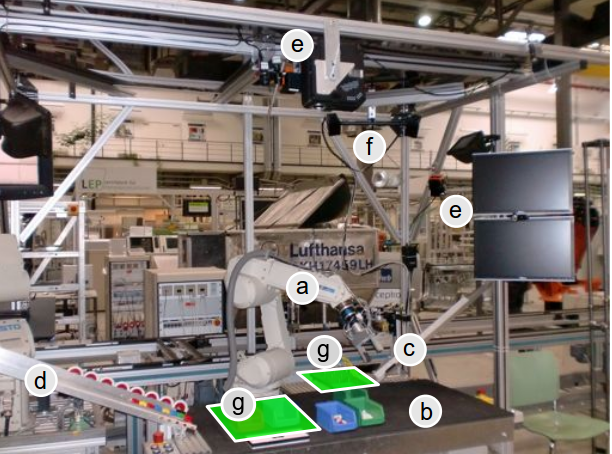
\includegraphics[width = 0.62\textwidth]{jahir.png}
\captionof{figure}{JAHIR assembly demonstration platform - a) Industrial Robot, b) Shared Workspace, c) Slide for Assembly blocks, d) Slides for Other Parts, e) Sensor Devices for Input/Output, f) ARTrack System g) Storage Space for Robot. Image from \cite{lenz2011}.}
\label{figure:jahir}
\end{center}

However, in reality, it is not feasible for assembly workers to wear a plethora of wired sensors while performing tasks. The physical and mental comfort is greatly reduced under such conditions, with the sensors creating a feeling of intrusiveness. A viable solution to this issue is the use of occupancy maps, which are commonly employed in robotics to determine position and motion, providing a robust approach to spatial perception and navigation problems. This technique, covered in depth in \cite{elfes1989}, was implemented for the robot assisted assembly task in \cite{lenz2011}, using the three-dimensional velocity, acceleration and jerk as input to the individual HMMs. This allowed for a recognition accuracy of 92.26\% for the right hand, comparable to the recognition rate of the reference experiment that relied on sensors. Therefore for the vast majority of the time, the system could accurately predict the task progress, and respond with the correct actions accordingly.


The key here is that the robot must be context-aware. This enables much greater cognitive capabilities and a higher standard of interaction with the user. Cognitive Technical Systems (CoTeSys) is a group with a research focus on sensing and actuation in the physical world. As explained in \cite{buss2010}, this allows the robot to exhibit behaviours that suggest it can `learn'. The foundations of cognition in humans and animals are used to develop cognitive models, which can then be applied when designing control systems for more specific technical applications. 

The group uses a cognition-based perception-action closed loop as a basis for investigating cognition in technical systems, as illustrated in Figure \ref{figure:cognitivearchitecture}. This architecture focuses on five main areas; perception, action, knowledge, learning and reasoning. The model may be directly applicable to the field of handheld robotics. Task knowledge and the way in which the device receives and processes data from both the environment and the user, acting accordingly, bears great parallels to the goal of handheld robotics in general. Thus this architecture may be considered as a reference when designing applications for handheld robotics. 

\begin{center}
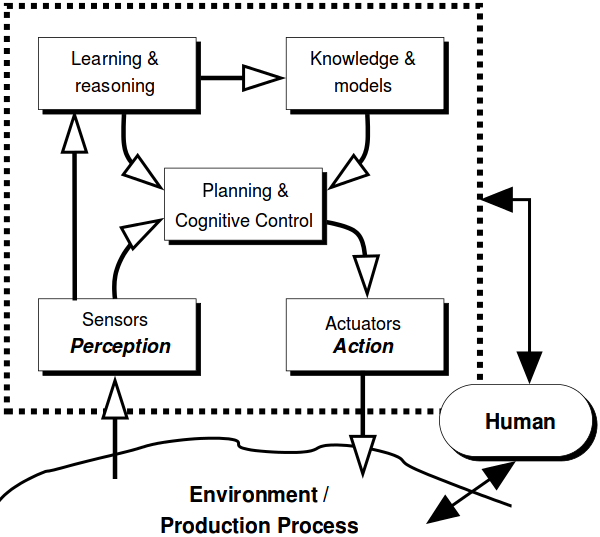
\includegraphics[width = 0.5\textwidth]{cognitivearchitecture.png}
\captionof{figure}{Cognitive System Architecture: Perception-Action Closed Loop, image from \cite{buss2010}.}
\label{figure:cognitivearchitecture}
\end{center}

\pagebreak














\subsection{Robotics in Building Environments} \label{building}

From a fully autonomous perspective, using robots in construction environments is becoming an increasingly attractive proposition. Although machines have been utilised to assist in construction since the industrial revolution, there has typically been few elements of automation. With advances in robotics, they may be incorporated into building applications to reach unprecedented levels of speed and efficiency. Numerous investigations and demonstrations have been carried out of robots performing assembly operations from a set of known requirements, corresponding to `task knowledge'. However, most of these examples are based around two-dimensional systems, such as manipulating blocks to construct flat structures, as in \cite{werfel2006}, not considering height.

\subsubsection{Mobile Robots} \label{mobilerobots}
Petersen et al \cite{Petersen2011} present a hardware system in which a mobile robot manipulates blocks in three-dimensional space to match desired structures. As well as this, they also produced a high-level control scheme that could enable multiple robots to autonomously share the workload of a user-specified building task. The results were successful and the prototype robot constructed structures that were greater in height than itself, doing so via climbing, navigation and manipulation. This was accomplished without the need for complex sensing and control mechanisms by the design of the simplified interconnecting structural blocks and the way in which the robot interfaces with them, as illustrated in Figure \ref{figure:buildingrobot}.

\begin{center}
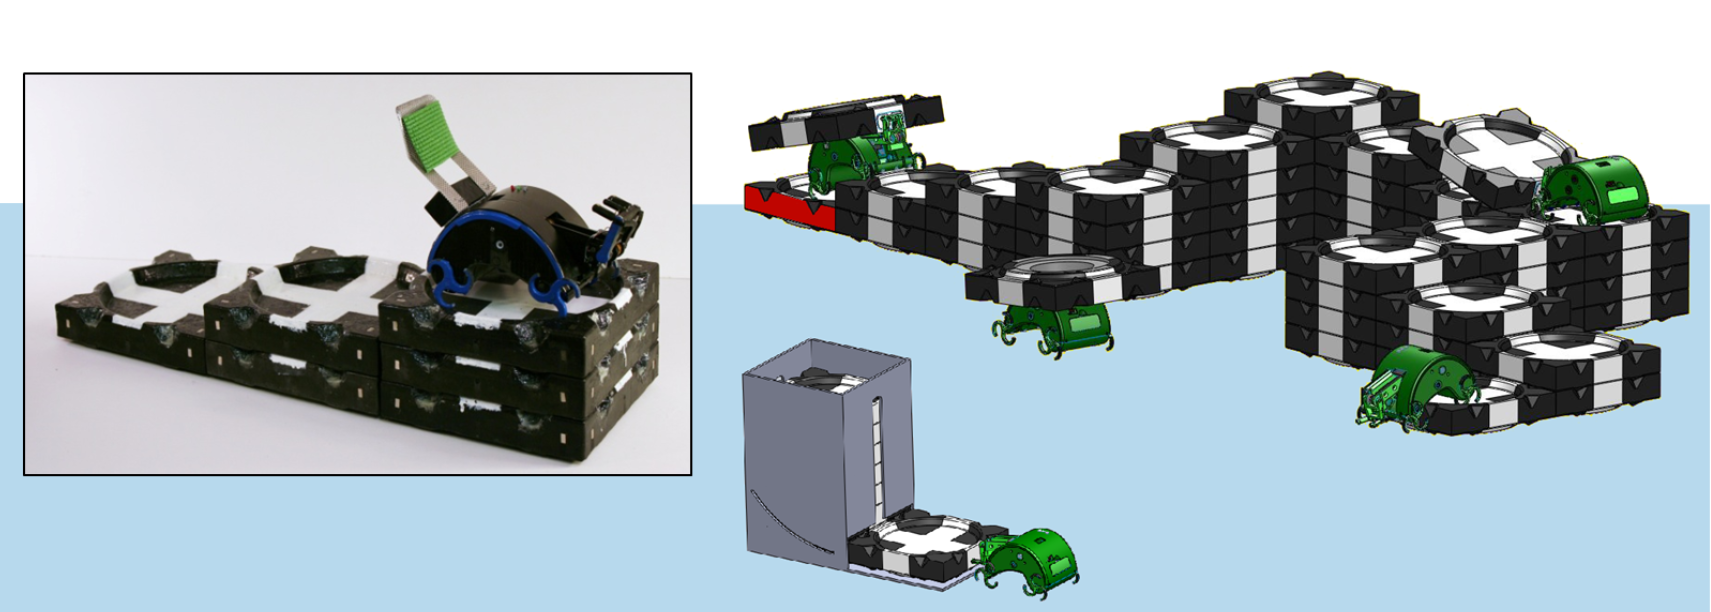
\includegraphics[width = 0.6\textwidth]{buildingrobot.png}
\captionof{figure}{Hardware system in which robot builds specified structures. Inset: Physical image of prototype atop six-block stricture. Outer image: Concept for system goal, in which multiple robots act together to distribute workload of a much larger structure. Image taken from \cite{Petersen2011}.}
\label{figure:buildingrobot}
\end{center}

This idea of designing the structure blocks in a passive manner so that they naturally fit together, reducing sophistication in orientation, provides a neat solution to overcoming positional errors. As such, inspiration will be taken from this general idea for the current experimental design, potentially also incorporating magnets for easy interaction. However, the blocks will have to be of a much larger scale and more plentiful, thus cost reduction in terms of material and manufacture will be a large consideration.

\subsubsection{Drone-Based Assembly}
With recent developments in Unmanned Aerial Vehicle (UAV) technology as a whole, it is becoming increasingly viable to deploy rotary wing platforms to interact with the physical environment. The main advantage they offer over typical ground based alternatives is improved speed and accessibility with regard to hard-to-reach regions. Moreover, using rotary wing based UAVs, such as quadcopters, over their fixed wing counterparts, allows for a more controlled operation in a tighter workspace. The design and control associated with transporting a payload with such a rotary based UAV is presented in \cite{mellinger2011}. The paper looks at different gripper designs and how successful the robot was in estimating and manipulating the mechanics of the varying payloads. Several issues arise when using UAVs to transport payloads, namely the limited weight bearing capacity and the fact that the dynamics are altered when carrying payloads. 

The grippers investigated in this paper either operate by traditional clamping (impactive) or surface penetration (ingressive). However, the reduced motion of the fixed claws inevitably leads to more positional uncertainty during hovering. A solution is proposed in \cite{cano2013}, which covers the design of a 6-DoF aerial manipulator (see Figure \ref{figure:uavmanipulator}) for UAVs to assemble bar structures. This is made possible by developments in high power aerial platforms, reducing weight restrictions. The 6-DoF manipulator in the paper focuses on three main functions; the \textit{capture} (approaching and grasping the bar), the \textit{transport} (transferring load from storage to site) and the \textit{assembling} (installing to the structure). Although this design remains relatively untested in terms of control, it possesses similarities to the handheld robotics design (similar DoF but contains roll), and inspiration may be taken when designing a new end effector for assembly-based tasks. The new end effector must be designed in tandem with the assembly blocks, and each of impactive, ingressive, rollers or passive-jointed magnets are viable options at this stage.

\begin{center}
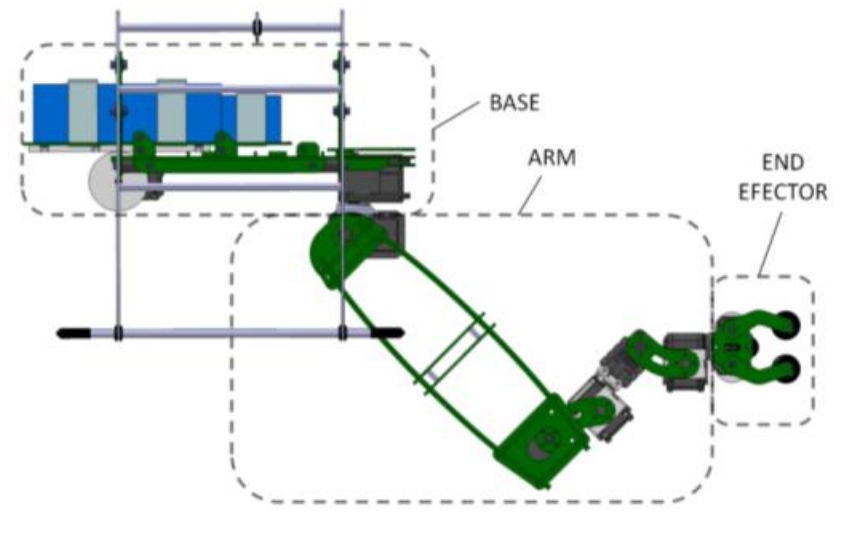
\includegraphics[width = 0.5\textwidth]{uavmanipulator.png}
\captionof{figure}{Components of Aerial 6-DoF Manipulator: Base, Arm and End Effector. Image taken from \cite{cano2013}.}
\label{figure:uavmanipulator}
\end{center}

The feasibility of using rotary UAVs to construct building-scale structures is explored in \cite{latteur2015}. In this paper, a project is outlined which envisions an alternative construction approach similar to that witnessed in nature; gradually adding more material to an existing structure in a safe and precise manner. Despite the energy considerations, it was concluded that large-scale construction may be possible through drones, with the potential improving in parallel with developing drone technology. An issue that was identified, as was the case in Section \ref{mobilerobots}, is the level of precision required for typical construction that is finer than afforded by fully mobile robots. This is even more evident in aerial vehicles. A similar solution was employed, allowing positional imprecisions through the use of modular self-aligning components. Three different approaches were investigated for such a component; \textit{droxels}, conical interlocking \textit{dricks}, and rounded conical interlocking \textit{dricks}. These designs provide further inspiration for designing the assembly components for the handheld robotics construction task.
\begin{itemize}
\item{Droxels (Drone Voxels) - Voxels are three dimensional pixels, different designs can lead to strong space-filling capabilities and allow for construction of complex shapes. They are somewhat more difficult to grasp and position but possess strong potential. One of the key issues is the manufacture complexity, with 3D printing being the most viable. See Figure \ref{figure:droxel}.}
\item{Conical Interlocking Dricks (Drone Bricks) - This option allows greater flexibility regarding positional tolerance. A lot of their potential lies in the fact that they can easily be constructed from more rigid structures such as concrete. However, unique blocks have to be designed to allow cornering. See Figure \ref{figure:cid}.}
\item{Rounded Conical Interlocking Dricks - Similar to the standard counterpart, except with a rounded shape and two full cones on top to allow for curved walls. See Figure \ref{figure:rcid}.}
\end{itemize}



\begin{center}
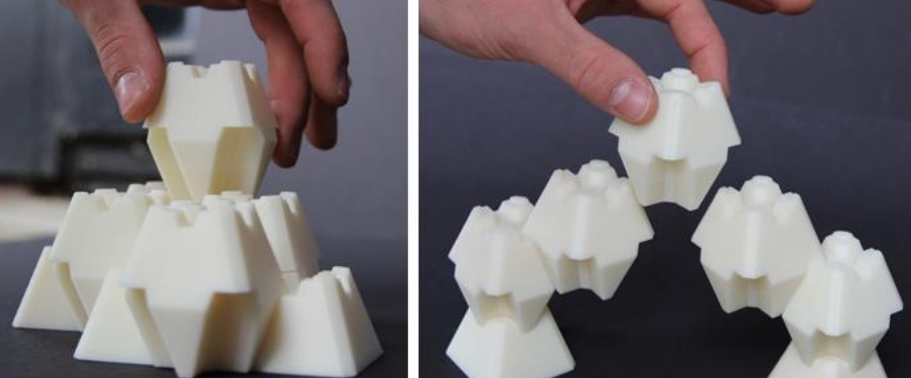
\includegraphics[width = 0.5\textwidth]{droxel.png}
\captionof{figure}{Droxel Design, image taken from \cite{latteur2015}.}
\label{figure:droxel}

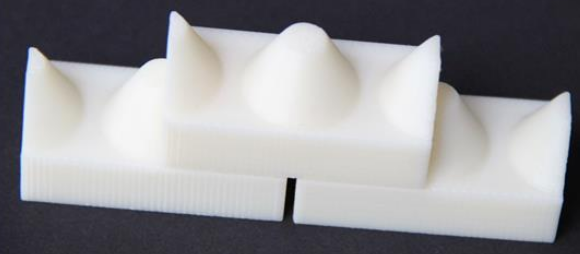
\includegraphics[width = 0.5\textwidth]{cid.png}
\captionof{figure}{Conical Interlocking Drick (CID), image taken from \cite{latteur2015}.}
\label{figure:cid}

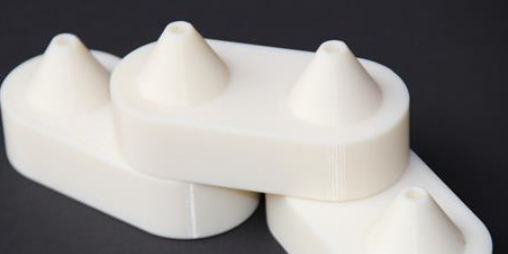
\includegraphics[width = 0.5\textwidth]{rcid.png}
\captionof{figure}{Round Conical Interlocking Drick (RCID), image taken from \cite{latteur2015}.}
\label{figure:rcid}

\end{center}



\subsubsection{Scene Knowledge}
One of the key considerations in robots performing construction tasks is how they navigate around the environment. The careful pre-planning of the construction environment is often necessary, so that autonomous agents can be informed of valid paths to avoid undesired collisions. Whole studies have been dedicated to this area, such as in \cite{Arkin1990}. In this paper, the autonomous agents are given prior knowledge of the environment as a whole and not just specific paths. This behaviour-oriented approach encourages vision/ultrasonic sensing to detect obstacles, reducing reliance on dead-set routes. Being more than fifteen years old, such techniques have become more established now, as in \cite{Petersen2011}. In many situations however, there is still a relatively strong dependency on a well defined environment, beyond just the relative locations of source/targets.

This reliance on environmental knowledge, as well as pre-planning of paths, is one of the areas in which handheld robotics can excel, providing an elegant solution to the guidance issues experienced by separate and autonomous robotics. As a user can transport and orientate a handheld robotic tool in any way they intuitively see fit, this mechanism provides much greater flexibility. The need for a rigidly defined environment and careful pre-planning, which is imperative to external robots, is vastly reduced with a handheld device. Of course, fixed obstacles can still be made known in order to provide the most efficient movement. However, as the user is in full control of the general location of the robot, the user actively recognises and avoids obstacles with virtually no cognitive effort. Hence this is an element of construction based robots that is of far less concern when designing the new experiment, further outlining the potential for handheld robotics as a whole. 

\pagebreak












\subsection{Handheld Robotics} \label{handheld}
\subsubsection{Medical Devices}
The field of handheld robotics has been largely unexplored in comparison to the established areas of robotics in which it sits between; fully external and wearable technology. The vast majority of the existing work in the handheld area is focused on the medical industry. Numerous surgical devices exist within this area, supplementing the skill and performance of the surgeon during precise operations. Payne and Yang \cite{Payne2014} review the existing and emerging trends in handheld medical robots, stating that the technical challenges differ from grounded robots in that miniaturising the devices is essential, whilst having multiple degrees of freedom is often less important.

An example of such a device is the handheld master-slave combined manipulator (MCM), developed by Matsuhira et al \cite{Matsuhira2002}, which offers added functionality to laparoscopic surgery that is not possible with conventional instrumentation. The design entails the addition of two degrees of freedom to the typical forceps, forming a cable-driven slave hand controlled by a master grip mechanism that houses two servo motors, as illustrated in Figure \ref{figure:masterslave}. The added yaw axes and the gripper end effector then enable internal suturing tasks, where potentiometers on the master grip interface with a notebook computer for controlling the motors. Other handheld robotics in the medical field include cutting implements incorporating haptic feedback (indicating force exertion) \cite{Payne2015}. There is also a significant amount of work regarding self-stabilising devices to compensate for physiological tremors, such as the  "ITrem" \cite{Latt2009}, which utilises sensing, filtering and manipulation to enhance surgical precision, or the mechatronic cup holder that alleviates the symptoms of Parkinson's patients \cite{Fischer2010}.

\begin{center}
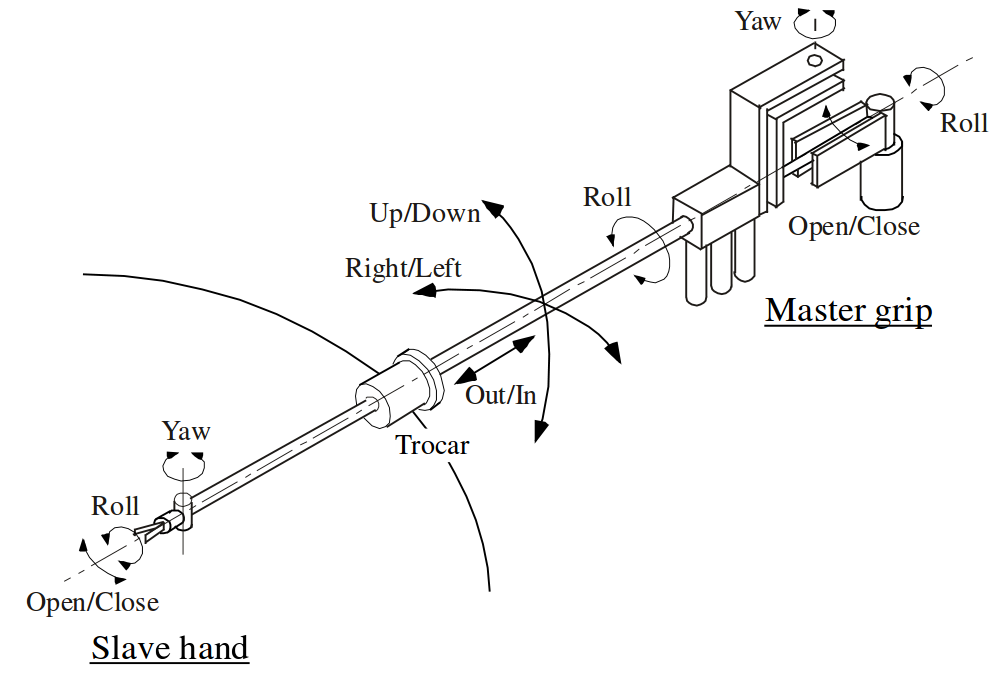
\includegraphics[width=0.5\textwidth]{laparascopic.png}
\captionof{figure}{Master-Slave Manipulator for laparascopic surgery, image from \cite{Matsuhira2002}}
\label{figure:masterslave}
\end{center}

However, up until 2015, there had been little research in the way of handheld robotics in the \textit{toolspace}. Tools have become a fundamental part of the way humans interact with the physical world, enabling the completion of tasks which would otherwise propose physical or mental challenges. They often allow operations to be performed that would otherwise be impossible, or simply reduce the task duration and workload, thus leading to an improved quality of life. One such example of work in this area is a handheld automated welding device, which enables welding to occur only when positioned correctly \cite{Echtler2004}. Although this constitutes an application of handheld robotics in the tool space, it is constrained by similar limitations to those present in the examples cited above when looking to classify this as a generalised handheld robotic tool that cooperates with the user. The aforementioned novel devices were designed with relatively few degrees of freedom and with very specific tasks in mind. This means that they are limited to single tasks, and cannot easily be adapted to alternative applications. The other key factor associated with the existing devices is their limited 'task knowledge', reducing the potential for cooperation between the device and the user.

\subsection{University of Bristol Handheld Robotics Project} \label{bristolhandheld}
\subsubsection{Initial Work}
Recent work undertaken at the University of Bristol has formulated the “Bristol Handheld Robotics Project”. This has focused on the potential of multi-degree-of-freedom handheld robotic devices operating in the tool space. A critical component of the research has been the capability of the robot to assume task knowledge for the desired procedure. The foundation for this branch of work was laid by A.Gregg-Smith and W.W.Mayol-Cuevas in \cite{GreggSmithDesign}, where a handheld robot was constructed and evaluated in terms of user cooperation. The underlying motivation of the paper was the assertion that there exists a much greater potential for handheld robotic applications than just the medical industry.

The work in \cite{GreggSmithDesign} covers the development of a four degree-of-freedom (4-DoF) prototype handheld robot, in which the aim was not to design a robot which can surpass human capability, but rather to evaluate the cooperation between the user and robot for various degrees of autonomy. This design and evaluation here has certainly laid the groundwork for future development of handheld robotics. The arm comprises a carbon-fibre backbone, and is cable-driven by two pairs of motors and pulleys located in the base; one opposing pair providing a degree of freedom each to the midpoint and the tip, with the other pair providing a second degree to each point, as illustrated in Figure \ref{figure:mark1}.


\begin{center}
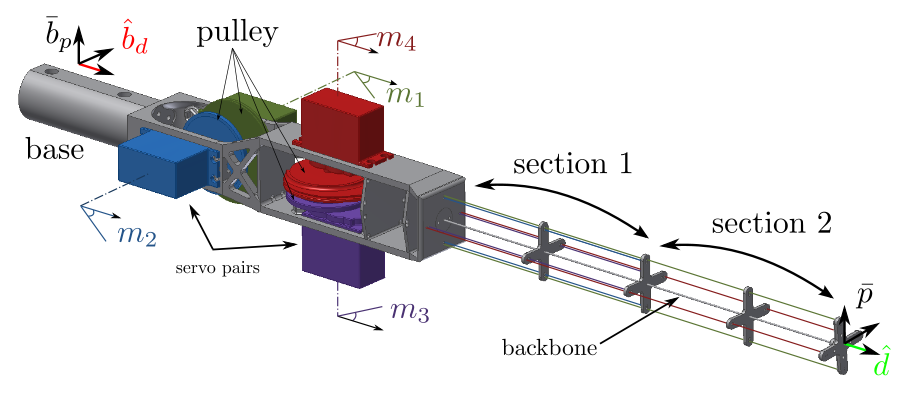
\includegraphics[width = 0.6\textwidth]{images/mark1.png}
\captionof{figure}{CAD model of the Four Degree-of-Freedom Mark I robot, image from \cite{GreggSmithDesign}.}
\label{figure:mark1}
\end{center}

The design takes inspiration from [31] which, unlike typical cable-driven designs, employs one motor
to provide tension to a pair of opposing wires, which reduces the the motor count to DoF ratio from 3:2 to 1:1. 
An external computer is used to interface with the servomotors and the trigger, responding to external
cues or program instructions by providing the necessary motion. In order to locate the robot spatially, an optitrack system made up of six strategically mounted cameras is
used to provide motion tracking, identifying the retro-reflective markers mounted on the robot. This
provides an accuracy of 0.2mm, although it was stated that the future aim would be to employ
on-board sensors for portability and practicality.


In order to calibrate the robot, it was necessary to perform kinematic modelling. Conventional forward
kinematics methods were not applicable to this design due to the non-linear interaction between sections 1 and 2
of the carbon-fibre backbone, shown in Figure \ref{figure:mark}. As such, a regression based method was employed.
This entailed sending a wide range of commands to the arm and recording the resulting pose with the
motion tracking equipment. In total, 14641 vectors of motor angles were sent, with the corresponding
poses comprising a relative tip-to-base position and direction. A Nadaraya-Watson kernel regression technique
was then used on the results to interpolate between the points to acquire pose estimated for unrecorded
motor vectors. 

MENTION K-D TREES HERE FOR ACCELERATED SEARCH AND IMPROVED COMPUTATIONAL TIME, OR MENTION IT LATER ON IN THE CALIBRATION SECTION AS AN OPTION AND FUTURE IMPROVEMENT????XXXXXX


It is important to note that due to the limits
of the carbon-fibre backbone, the arm cannot self-intersect, therefore it is safe to interpolate
between the motor angles.

Inspiration was taken from this Mark I design in the development of the newer, flexible tube-based model, and naturally, similarities will be observed between the set up and control processes and the external infrastructure to interface with the robot and provide track motion. The key differences originate from the different arm material/structure, having a chain reaction of required design changes. Also, with the benefit of hindsight, design and material choices that hindered this Mark I design could be avoided, while strong points could be adapted. An example of this is the issue of the friction from the cables wearing through the base material. This led to the choice of an ultra low-friction cable material, and a stronger base material, using PLA over ABS. 

ALSO MENTION SIMILARITIES WITH THE TLX STAGE IF ANY OF THIS GETS COMPLETED IN PRACTICE XXXX

 , as well as the techniques used to quantify the task performance an perceived effort. 



\subsubsection{Development of the 6-DoF Handheld Robot}

A second robot was designed and built, offering two extra degrees of freedom over its predecessor, as covered in depth in \cite{GreggSmithKinematics}. The key difference between the two designs is the way in which the degrees of freedom are enabled. Whilst the first design comprised flexible backbone, the updated version possesses six links, as illustrated in Figure \ref{figure:links}. The design takes inspiration from the 2.4m long Mini 3D CT-Arm \cite{Horigome2014}, with modifications and a shorter arm length (30cm) to make it suited to handheld applications. These links allow for a much greater range of motion, with each link individually driven by a pair of cables connecting the corresponding motors to the link driving pulleys (located on the link).

\begin{center}
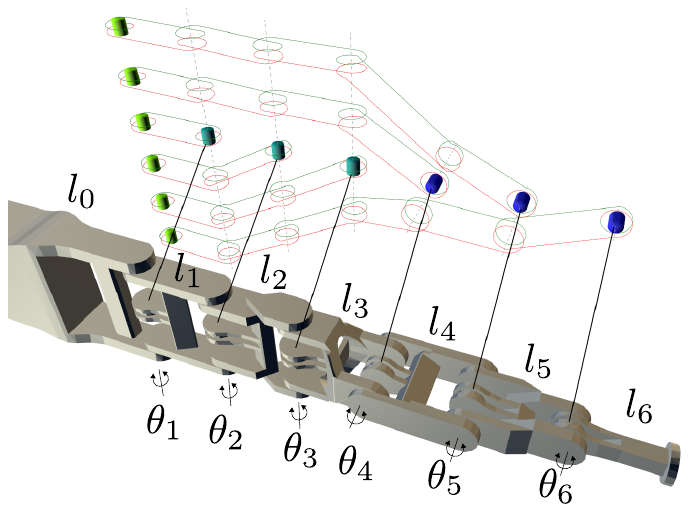
\includegraphics[width = 0.6\textwidth]{links.png}
\captionof{figure}{CAD model of arm, with motor pulleys and link pulleys represented by the green and blue/turquoise cylinders respectively. Links are represented by \(l_0\) to \(l_6\) and joint angles by \(\theta_1\) to \(\theta_6\). Image from \cite{GreggSmithKinematics}.}
\label{figure:links}
\end{center}

The design covered in \cite{GreggSmithKinematics} employs a system which allows a single DoF to be controlled by a single motor, thus six Dynamixel servomotors are mounted at the base. However, to prevent slippage in this design, the motors are mounted on cable tensioning mechanisms which can be individually located by a lead screw. As such the robot must be re-calibrated whenever re-tensioning the cables. A 3D space carving analysis was performed on the design of the links, which consisted of looking at the two extremes of the neighbouring links and identifying the volume of the link they would not sweep away. This allowed the range of motion of the arm to be maximised and the mass of each link to be minimised. Combining these analyses with ergonomic considerations resulted in a lightweight, tentacle-like design, improving on the rigidity and motion capabilities of the first prototype. The design in its entirety is illustrated in Figure \ref{figure:mark2}, and is made open-source at \cite{handheldrobotics}.

\begin{center}
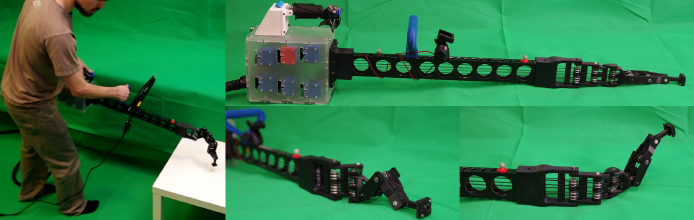
\includegraphics[width = 0.6\textwidth]{mark2.png}
\captionof{figure}{MK II handheld robot design, image from \cite{GreggSmithKinematics}}
\label{figure:mark2}
\end{center}

Due to the increased numbers of degrees of freedom and the range of motion, the kinematics are more complex to implement in this design. One crucial difference with the two designs is that current version is built such that the links may self-intersect at certain joint angles. As covered in \cite{GreggSmithKinematics}, when moving from one specific position to a target, a path planning algorithm was used. The input to this planner is the target angles of each of the motors so that the required pose may be obtained. Due to the nature of the robot, there are often multiple combinations of valid motor angles that would result in the necessary end effector pose. This implies that some positional vectors of the motors would act as more suitable inputs to the path planner than others, producing more efficient paths.

General purpose inverse kinematic solutions, such as that provided in \cite{Aristidou2011}, were considered for applying to the robot. However, due to their computationally intensive nature, and the fact that they generally return only one solution, a different approach was opted for; an analytical solution. This would provide a range of valid options, allowing the path planner to select the optimal configuration for the given situation. 

This analytical approach in \cite{GreggSmithKinematics} entailed splitting the kinematics into two 3 DoF problems; for the first three links (same horizontal plane as base) and the last three links (same vertical plane as end-effector), with the central link \(l_3\) acting on a line common to both planes, as illustrated in \ref{figure:kinematicsDof}. Seven boundary constraints were then defined for the first problem, which cover all self intersections and the maximum angles of each joint, based on a known direction of the central link and the location of the first link. Once solved, the same approach was taken for the second problem, only using the location of the end effector link instead of the first link. The solutions generated from each set are then merged, with the overlaps giving suitable configurations. 

\begin{center}
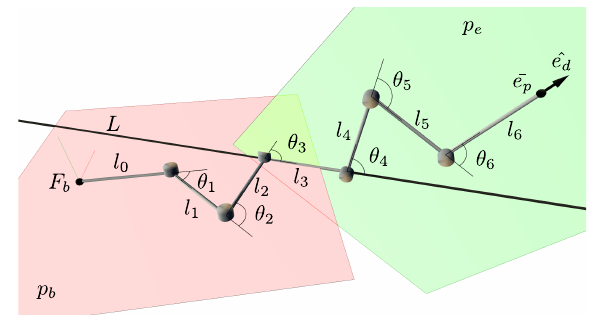
\includegraphics[width=0.45\textwidth]{kinematicsDof.png}
\captionof{figure}{Splitting the kinematics problem into two using a different shared plane for each set of links, with link \(l_3\) acting on a common line. Image taken from \cite{GreggSmithKinematics}.}
\label{figure:kinematicsDof}
\end{center}

The resulting set of valid configurations can then be passed into the path planner, which plots a suitable path. This may entail using the quickest possible route based on the current location, or an alternative route to avoid collision with a physical obstacle. In certain situations, the desired end effector pose may not be possible based on the current location. In such an event, a `graceful degradation' approach was introduced in \cite{GreggSmithKinematics}. This entails getting as close to the target as possible, which may mean achieving the tip position but not the direction. Or, in cases where the target is simply too far away, the arm will `point' to the desired location. As the correct pose moves further away, the robot will reduce the active degrees of freedom to get closer. This appears intuitive to the user in that the degree of distance away from the current location is represented by how `straight' the robot appears to point.

This is directly relevant to the current project in that this will be the robot used for the experiment and user study. The kinematic method, of checking within the specified boundary conditions and selecting from a range of suitable positions for the central link, will be employed to ascertain necessary motor configurations. Thus it is essential that this is well understood, as all physical operations will rely on it and it will indicate why something has succeeded or failed. Furthermore, the protocol of the Dynamixel MX-64T servomotors \cite{DYNAMIXEL} must also be researched as it will be interfaced with (using C\#) in order order to program specific motions to the robot.

\subsection{Designing Experiments for Handheld Robotics} \label{designingexperiments}
At such an early stage in the development of handheld robotics, it is essential to carry out well designed experiments that reveal as much as possible about the various aspects of the field in general. Focus must be placed on important factors such as how well the user and device cooperate, how the desired actions of the robot are communicated to to the user and the benefits of using the device in terms of perceived effort and performance. The earliest experiments undertaken focused on evaluating the cooperation of the human and robot. Other experiments include investigating the effectiveness of different feedback methods for the robot in communicating desired positions, as well as the kinematics and motion in general.

\subsubsection{Painting Task}
The painting task from \cite{GreggSmithDesign} entailed users being shown a template pattern on a screen and assigned with going over the pattern with ``virtual paint". The motion capture system would register the position and direction of the tip of the arm and the key action would result in virtual painting, painting the pixels the tip is pointing to. 

In both manual and semi-autonomous mode, the key action was the user pressing the trigger to initiate painting. The semi-autonomous mode draws upon the robot's task knowledge to enable movement among contiguous pixels in the same target region while the trigger is held. However, it cannot move across gaps to unpainted regions by itself. Alternatively, the fully autonomous mode involves the robot initiating and halting the key action itself, moving and painting where it deems appropriate, as illustrated in Figure \ref{figure:painting}.

\begin{center}
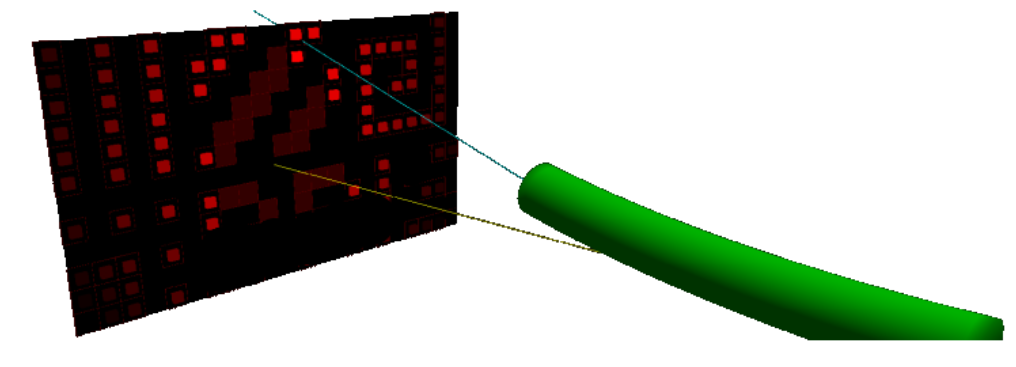
\includegraphics[width=0.5\textwidth]{painting.png}
\captionof{figure}{Model of painting task setup in autonomous mode (lights indicate preference of next motion), image from \cite{GreggSmithDesign}}
\label{figure:painting}
\end{center}

\subsubsection{Tiling Task}
The tiling task from \cite{GreggSmithDesign} involved fitting the end-effector with an electromagnet and picking up red or black tiles from designated hoppers before placing them in a predefined chequerboard pattern, as illustrated in Figure \ref{figure:tilingtask}. The magnet is activated/deactivated by pressing the trigger, except in the case of full autonomy in which the robot has full control of this key action. In the manual mode, the absence of task knowledge means the arm remains straight and its only actions are responding to the trigger press with the magnet. In this case, it is possible for the user to create an erroneous pattern, so a template was made visible so that all users performed the task correctly. 

In the two modes that comprise task knowledge, the arm will move towards the nearest hopper that will provide a suitable colour, and then move towards the nearest suitable empty space on the board. In both cases, the robot will refuse to perform an action that conflicts with the task specification. In the case of full autonomy, the electromagnet is also controlled by the robot. Thus the tool will keep seeking to perform necessary actions, gesturing to the user where it should be positioned to do so, until the task is complete.

\begin{center}
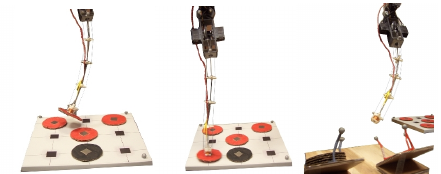
\includegraphics[width=0.5\textwidth]{tilingtask.png}
\captionof{figure}{Pick and Place Tiling Task with tip of first prototype, image from \cite{GreggSmithDesign}}
\label{figure:tilingtask}
\end{center}

The results from the previous two tasks indicated that the completion time was significantly improved with increasing degree of autonomy. The accuracy of the tasks however, showed little difference among the different modes. This was to be expected as the robot end effector was designed with an accuracy comparable to that of a human. The combined TLX scores also showed improvement with increasing autonomy, indicating that cooperation with the robot reduces the perceived task effort. The individual TLX scores for various factors are shown for both tasks in Figure \ref{figure:tlxscores}.

\begin{center}
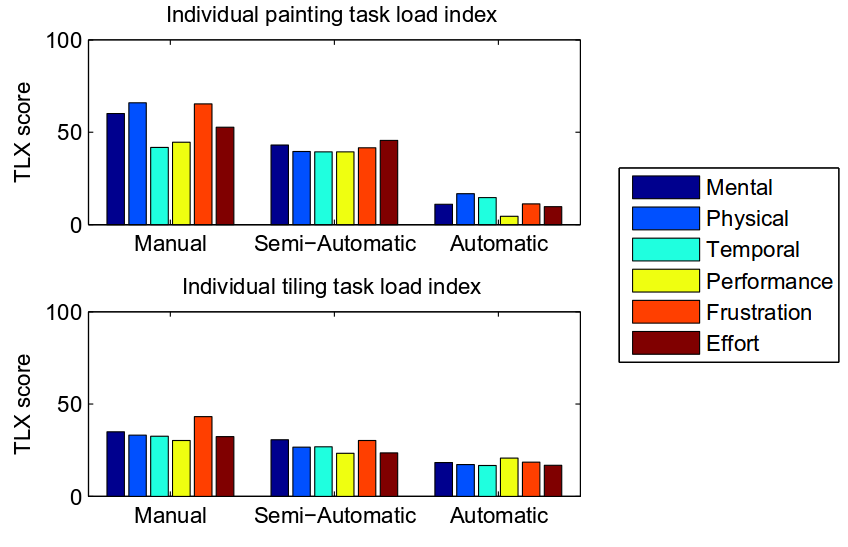
\includegraphics[width = 0.455\textwidth]{tlxscores.png}
\captionof{figure}{Individual TLX scores for both the tasks, image from \cite{GreggSmithDesign}}
\label{figure:tlxscores}
\end{center}

As the task accuracy exhibited little difference among the modes, and the completion time and perceived effort showed improvement with task knowledge, it was concluded that the users cooperated well with a handheld robot with task knowledge, where introducing levels of automation had a positive impact on essential elements of task performance. Although sharing elements of the task among the user and robot did not negatively affect performance, maximum benefit was attained when the robot was given full control. Of course, there is still a strong element of cooperation in this scenario as the user must move the robot to its desired location, responding to its gestures.
	
\subsubsection{Spatial Guidance Task}

Manoeuvring the robot to a specific location so that it may perform its duties is an essential element of a strong cooperation. Without effectively conveying desired locations in order to proceed with the task, the usefulness of the robot is severely hindered. Thus, some form of guidance is necessitated. Fitt's law is an established method of estimating the time to reach a known destination \cite{fitts1954}, and although was originally created with a 2D perspective, it has been extended to a 3D environment, such as in 3D pointing tasks \cite{Cha2013}. In either case, the way in which information is presented to the user from a human interaction point-of-view has often been considered to affect performance \cite{soukoreff2004} \cite{MOTOYUKI1995}. 
  
As covered by A.Gregg-Smith and W.W.Mayol-Cuevas in \cite{GreggSmithFeedback}, various methods were investigated in which the robot provided spatial feedback to the user during a 3D guidance task. The task comprised positioning the robot so that the end effector could be aligned to within 5mm and 5 degrees of a target pose for at least 200ms. The target pose took place at a range of locations on a small side table, and was also performed using a handheld wand in order to evaluate the benefit of using the robot.

The seven conditions investigated are listed below, with the experimental set-up for the robot with virtual reality illustrated in Figure \ref{figure:vrrobot}.
\begin{enumerate}
\item{Robot provides gestures by pointing to location}
\item{7 inch 2D screen mounted to robot, showing wireframe model of table and target point}
\item{7 inch screen held in one hand, performing task with wand in other hand}
\item{Augmented reality headset (with transparent lense) while using robot}
\item{Augmented reality headset while performing task with wand}
\item{Virtual reality headset while using robot}
\item{Virtual reality headset while performing task with wand}
\end{enumerate}

In each case, an infra-red optical tracking system was used with retro-reflective markers attached to the key objects; the arm, wand, table, augmented/virtual reality headsets and the 7 inch screen. This allowed a 6-DoF pose of the robot to be calculated.

\begin{center}
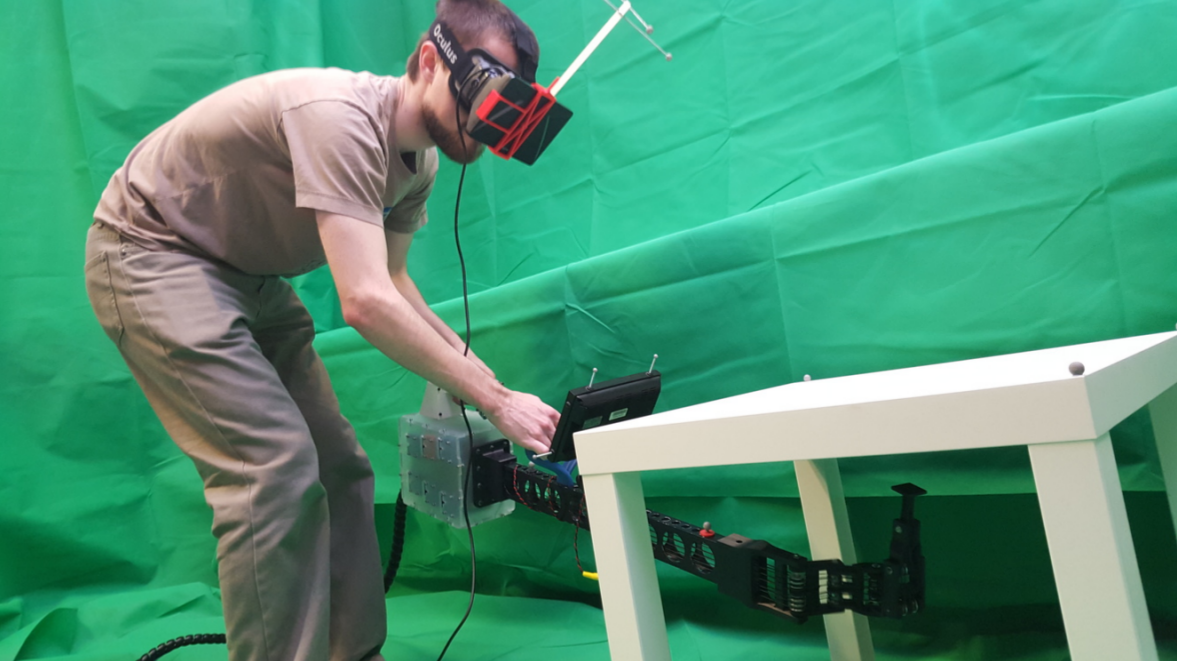
\includegraphics[width=0.55\textwidth]{vrrobot.png}
\captionof{figure}{Spatial guidance task being performed with the handheld robot where feedback is provided via a virtual reality headset, image taken from \cite{GreggSmithFeedback}.}
\label{figure:vrrobot}
\end{center} 
 
The robot itself possessed a 6-DoF pose in world space, while the joint angles constitute a further six DoF, resulting in an overall 12-DoF pose. Solving from one of these fully defined poses to another is computationally expensive, requiring minutes to be calculated where sub-second times are needed for a responsive tool. In order to overcome this issue, the path planning ability of the human was exploited, resulting the robot path-planning problem to 3-DoF. A variant of informed Rapidly Exploring Random Trees (RRT*) \cite{Gammell2014} was then produced in \cite{GreggSmithFeedback} to calculate the shortest route from robot to target, using the frame of reference of the target as the root of the tree. Once such a trajectory is known, the robot can gesture along it as a feedback method, and also find the closest point to the user which has a 5-DoF inverse kinematics solution, as explained in \cite{GreggSmithKinematics}. This algorithm was always run during robot use, regardless of the feedback method.

The results of the completion time and the TLX combined scores in \cite{GreggSmithFeedback} indicate that the three forms of visual feedback (augmented reality, virtual reality and mounted screen) are shown to improve performance compared to the handheld wand. The gesturing mode of feedback does not show as great an improvement over the wand. However, there was little difference exhibited among the visual feedback methods when employed on the robot. The strong results demonstrate the effectiveness of the robot in assisted tasks, outlining its potential for use in the tool space.
	
\subsubsection{Added Value of New Experiment}
The objectives of the current project entail interacting with physical objects in a 3D representative environment, which differs from the physical interaction task performed in \cite{GreggSmithDesign}. The tiling task, although in reality involved relocating 3D objects, can be represented by a 2D environment. The task knowledge did not involve the depth of the tiles, and therefore they could be assumed to be a perfect disk with zero depth. The user would lower the robot until the discs were picked up or placed, whereas the two dimensions the robot focused on were in the x and y axes; lining up the end effector with the centre of the chequerboard positions.

Alternatively, this project aims to evaluate tasks performed in a 3D rich environment, interacting with objects of known width, height and depth, which must be placed accordingly to simulate a simplified construction environment. A different end effector will be designed, and although it may possess similarities to that used in the tiling task (electromagnet based) it will require an alternative mechanism to consider true 3D space. That is, the alignment of the objects will be important so the end effector must be such that different angles of approach will not cause alignment issues. Moreover, the work in \cite{GreggSmithDesign} focused more on generic tasks that would require no specific skill and be of little difficulty to the average person. As this project is investigating a more definitive scenario (building environment), the robot used in the new tasks will likely possess task knowledge and capabilities exceeding those of an unskilled worker. This coincides with the idea of enabling complex task completion by those without conventional training in that area, such as crowd-sourced building projects.

The spatial guidance experiment in \cite{GreggSmithFeedback} has yielded useful information regarding the development of handheld robotics in general, considering the importance of effectively conveying preferences to the user. For the current project, the guidance provided to the robot to the user will certainly play a big part in performing the experiment. This is especially so if mental attributes are added to the task to make it harder for the user to complete without assistance. Thus, if the tasks contain elements where the target objects are not immediately visible to the user, one of the three visual feedback methods demonstrated in this paper can be used with confidence. The use of the path planning algorithm in \cite{GreggSmithFeedback} to come up with a suitable 5-DoF pose will also be a key component of the new experiment.


\subsubsection{Task Load Index (TLX) and Perceived Effort}

When investigating task effectiveness, it is essential to quantify the perceived workload of the performer. This is especially true when researching methods that may improve the task performance. The established means of this quantification is the use of the NASA TLX (Task Load Index). A multi-dimensional scaling was introduced in \cite{hart1988} under the belief that subjective workload is in fact measurable, and has since become widely accepted. Subjective responses can thus be reliably evaluated to meaningful ratings. The six key rating scales associated with the index are mental demand, physical demand, temporal demand, performance, effort and frustration level. 

This TLX methodology was employed on each of the experiments that have been carried out for handheld robotics thus far \cite{GreggSmithDesign} \cite{GreggSmithFeedback}, yielding valuable information regarding the subjective workload of cooperative tasks with the robot. As such, it is logical that a similar technique will be used on the new experiment. An ethics approval agreement is already in place that will span the duration of the project. This will allow the undertaking of studies with human participants, concluding with them filling out a TLX form. 
\pagebreak




\section{Summary}
A review of existing literature was carried out in order to better understand the area in which this project aims to contribute to. Most notably, the current work regarding handheld robotics at the University of Bristol was looked into. This is especially relevant as it formed the groundwork on which this project will be based,  providing crucial details of the apparatus that will be used. Particular focus was given to the design process which has led to the robot's current state and the evaluations of its performance and cooperation. 

Coinciding with this is the kinematics information on which the current robot is based. It was necessary to understand this as the approach used for the robot control will need to be exploited to perform any task scenarios which make up the evaluation. The recent study on the methods of feedback for the robot in \cite{GreggSmithFeedback} has enabled confidence when choosing how best to convey spatial information to the user. This is of obvious importance, as the robot will have to interact with the user to to indicate where it should next be located during the task, regardless of the specifics of the experiment. It may also become more pertinent throughout the development, if objects are out of line of sight.

A brief review was performed of the field of human in-the-loop operation. Despite being mostly based around external robots that require human input, it still provides useful insight into the way that humans interact with shared robotic tasks. An area of interest that was found dealt with `sliding autonomy' in which the degree of autonomy the robot exhibits can be fine tuned in a system of transfer of control. This led to improvements in task performance by combining the efficiency of the autonomous agent and the reliability of the human perspective, aiming to determine an optimal balance. This may be worth investigating in the future as a means of potentially locating a more efficient degree of autonomy for certain tasks. 

Another approach taken dealt with the weighting of inputs, in which both the human and the robot provided an input, and the singular operational result was formed of a combination of the two. Although this may not be applicable to precise operations, the idea of weighing two inputs based on a current situation may prove beneficial in selecting the operation. For instance a human user could indicate somehow that the situation has changed and the robot must carry out a certain operation, regardless of the task specification.

Furthermore, a brief overview was provided for robots in construction related tasks. This proved to be rewarding in that papers were found that provide a simplified construction environment for testing, albeit on a much smaller scale. The idea of passive structure blocks which easily fit together will most likely be employed on the design of the experiment, and the methods in which the blocks were produced (foam cutting around a template) will also be looked at in detail as a cheap and effective solution. A number of alternative designs were found for such self aligning assembly blocks, providing a basis of inspiration for the new experiment.


\pagebreak
\pagebreak

\section{Handheld Robot Design}
\subsection{Flexible Robotic Arms}
\subsection{Design Process of Four Degrees-Of-Freedom Device}
\begin{itemize}
\item{The initial design took direction based on the use of four Hi-Tec MS7980 servomotors to provide a degree of freedom each, driving the arm via some form of lightweight cable.}
\item{A flexible foam tube was provided to act as the arm of the robot with outer diameter 42mm and inner diameter 19mm}
\item{Early design was based around a single solid part, where two servos were mounted at the back and another two slightly offset. A tubular section was also present to attach the foam arm. However, after attempting to 3D print this, the quality was severely hindered by the need for excessive scaffolding to support the overhanging elements of the design}
\item{As a result, the base was designed in two halves, with a separate piece for the tubular mount for the arm. These three parts could then be printed separately in an orientation that didn't result in any overhanging sections. As such, a much higher 3D print quality could be achieved.}
\item{At this point, alternate shapes were explored based around this fundamental design, with compactness being a priority. One such design would entail a cubic section, where all servomotors would be at the same level, reducing the required moment arm to hold the device}
\item{The cable management was then accounted for in order to drive the arm. Tubular linkages are attached to the arm with holes to connect the cables to the servomotors. When connecting the cables from the servomotors to the tubular linkages, the orientation of the cables in 3D space must be considered in order to determine how the arm will move in response to servomotor angle changes. Initially, the cables were planned to be connected in a straight line direct from the servomotor to the arm linkages, eliminating the need to account for friction}
\item{INSERT IMAGE OF THE CAD OF THE CUBIC DESIGN WITH CONNECTING LINES}
\item{However, by connecting the cables directly, in a manner with a relative angle between the axis of the arm, the motion of the arm in response to a servo angle change is unpredictable, and more importantly, a single servo motion may not necessarily constrain the arm to motion in a single degree of freedom. That is, the arm will move in one direction initially, resulting in a different angle between the cable and the arm, and further servo motion will cause movement along the axis of the cable (in a different direction to the initial motion). }
\item{As such, it was decided that a configuration was necessary that routed the cables so that each servo acts solely on a single degree of freedom, with the cables running parallel to the arm. This of course required changing the direction of the cables by passing them through guiding holes, accepting friction where they make contact with the edges of the holes.}
\item{Further iterations of the dimensions in the design were explored in order to find a configuration in which the cables of the rear pair of servos did not interfere at all with those of the front pair. Holes were implemented on the central tube holder pillar so that the cables could pass through in an orientation normal to the servo arms of the rear (so the driving force on the servo arm would be tangent to the radius  of the servo arm motion), meaning that motion from the servo would result in the maximum movement of the arm. If it was directed non-tangentially, motion from the servo would have less of an effect on the motion of the arm.} 
\item{PUT IN IMAGE OF SERVO ARM WITH CABLE ATTACHED TANGENTIALLY AND MOTION TO SHOW LARGE CORRESPONDING MOTION, AND THEN SIMILAR FOR ATTACHED AT AN ANGLE SHOWING LESS MOTION.}
\item{A similar approach was taken to guiding the cables of the front two servos by passing them through holes in the base mounting for the tube holder }
\item{Once the cables have been guided in such a way that they are perpendicular to the servo arms, they then required another set of holes in order to guide them along the axis of the arm. Therefore a faceplate with four guiding holes was fitted to the front of the housing.}
\item{A low friction fishing wire was thus selected as the cable material [INSERT REFERENCE TO PRODUCT??], and was found to move freely against the 3D printed PLA plastic with little signs of wear or grazing}
\item{An initial prototype was printed with relatively low percentage infill in order to test the concept. The medium sized servo arms that were supplied with the servo were used, feeding the cables through the set of holes along each side of the arm to lock it in place. Exiting the cable at the outermost hole gave an effective diameter (which acts on the cable) of 45mm, whereas the overall diameter of the servo arm was 52mm. Initially, this prototype was ran with all four servos connected to the respective arm linkages, achieving correct motion. This proved that the friction of the cables was not a cause for concern, and the routing of the cables was successful. However, the range of motion of the front two servos were limited by potential collision with the base mounting for the central tube holder, only affording 35 degrees either side of the neutral position. (the max range of the servos is 70 degrees either side but this should have been mentioned already.}
\item{Another issue found was the inconsistent rate of motion in a given degree of freedom with increasing servo angle, this is for similar reasons as explained earlier in FIGURE X [THE ONE SHOWING THE CABLE ATTACHED TANGENTIALLY TO THE SERVO ARM]. At larger angles, a similar movement of the servo arm results in a smaller response motion from the arm. Hence the effect is an overall reduced range of motion of the arm as high servo angles have minimal effect on the motion as they don't pull the cable further. The other key problem observed was that on the opposite side to the pulling action of the arm, the cable became slack. This is because as the arm flexes, the extra cable available afforded by the forward motion of this end of the servo arm [USE A DIFFERENT WORD TO ARM] is not made up by the increase in arc length on that side of the robot arm  as the cable itself does not follow the curve, but takes the  direct path between the two linkages, a distance which has actually become shorter as it will always be a maximum when the arm is straight [THE CABLE IS FED THROUGH THE MIDDLE LINKAGE ON WAY TO THE TOP OF COURSE, MENTION THIS EARLIER], [ALSO PUT IMAGE OF THIS EFFECT AND MAYBE REFERENCE AUSTIN PAPER AS SIMILAR EFFECT WAS OBSERVED}
\item{The latter problem was addressed by adding another pair of linkages that merely act to guide the cable, and are not driven unlike the other two. This reduces the relative difference of the distance the cable has to cover in normal and flexed states, thus reducing the amount of slack occurring.}
\item{Pulleys used to address other problem....}
\item{Dimensions changed to afford more room to front servo to allow it to move full range of servo motion.....} 
\end{itemize}
\subsection{Interfacing With NatNet Optical Tracking System}

In order to determine where in three dimensional space the robot is, as well as the relative distances between itself and other points, it is necessary to track physical objects. This was achieved using a single optical tracking device, the Optitrack V120 Duo [REFERENCE TO DATA SHEET XXX]. The device features two cameras in order to provide depth perception, and works as a stand-alone device unlike the syncing of several distinct cameras as used in \cite{GreggSmithDesign} and \cite{GreggSmithFeedback}. The accompanying software library however, the `NatNet SDK', as well as the actual tracking software, `Optitrack Motive', are the same. This library was provided to run in a .NET framework environment, hence the decision to use C\# as the primary development language.

The device recognises the supplied retro-reflective markers, and is able to provide six degrees of freedom tracking. It is important to not that the coordinate system used by the software is based around the positioning of the Duo tracking device itself, with the 

\subsection{Controlling The Device}
\subsection{Calibrating Device Using Kernel Regression Method}
\pagebreak 
\subsection{Algorithm for Responding to Three-Dimensional State Requirements}
Once the robot has been calibrated in such a way that there exists a suitable range of data points in which to perform the regression function, along with the selection of an appropriate bandwidth, the device may then be responsive to 3D state commands.
The process of responding to commands is fundamentally built on inputting a positional vector, an orientation vector or a combined vector into the regression function in order to ascertain the required motor angles. This input vector is of course in regard to the tip relative to the base, as is the corresponding calibration data. The resulting motor angle vector is then issued to the servomotors via the Arduino in a controlled manner. 

However, in order for this approach of obtaining servo angles from a given input to be useful in practice, it is first essential to determine the correct input to the regression function. This can depend on a variety of factors relating to the absolute 3D target point and its relation to the base of the robot, such as the current orientation of the base and the relative proximity of the target.

\subsubsection{Acquiring Target Position Relative to Orientation of Base}
The robot is fixed in place while the optical tracking software is configured to recognise the rigid bodies formed by the retro-reflective markers associated with the base and the tip, as covered in SECTION XXXXXXXX (just say 'is configured'?. At this point, the base is said to have zero orientation about any axis (as this was the point it was first initialised in). The calibration procedure is then of course undertaken while the robot is fixed in this position. Thus, the stored relative tip-to-base calibration data for different servo angle vectors is only valid for the robot in a zero orientation position compared to the starting position. Hence, in practice, when the base has changed orientation about any of the three axes inherent to the optical tracking device, a direct input for a relative tip-to-base position will yield incorrect motor angles to meet this position. Therefore, the target position must be adjusted in order to account for the varying orientation of the base.

The orientation of the base itself is initially stored as a quaternion within the rigid body object from the NatNet library \cite{natnet2016}. This is then converted to euler angles using a built-in method to represent the orientation as three angles about the tracking device's X, Y and Z axes respectively, of which the order is important. It is thus necessary convert a real target point to an equivalent point relative to the original orientation of the base (zero orientation), so that the regression function and stored calibration data can be used to yield angles that result in the correct relative position in real space. This is accomplished using a rotation matrix that accounts for the rotation ordering of the base. Given that the base orientation is represented by rotation about the X, then Y, then Z axes, the converted point will be attained by taking the actual target point relative to the base and reversing these rotation operations; that is, the negatives of the base rotation values about the Z, then Y, then X axes. The rotation matrix in figure \ref{equation:rotationMatrix} is thus used to account for this axes of rotation order. 

\begin{center}
\[
R_{x}R_{y}R_{z} = 
\begin{bmatrix*}
\cos\beta\cos\gamma & -\cos\beta\sin\gamma & \sin\beta \\
\cos\alpha\sin\gamma + \sin\alpha\sin\beta\cos\gamma & \cos\alpha\cos\gamma - \sin\alpha\sin\beta\sin\gamma & -\sin\alpha\cos\beta \\
\sin\alpha\sin\gamma - \cos\alpha\sin\beta\cos\gamma & \sin\alpha\cos\gamma + \cos\alpha\sin\beta\sin\gamma & \cos\alpha\cos\beta \\
\end{bmatrix*}
\]
\captionof{figure}{Rotation Matrix for rotation about Z, then Y, then X axes. The symbols $\alpha$, $\beta$ and $\gamma$ represent rotations about the X, Y and Z axes respectively, adapted from \cite{3drotation}.}
\label{equation:rotationMatrix}
\end{center}

A simplified example of solving from a target point to get the appropriate relative positional vector as an input to the regression function is illustrated in Figure \ref{figure:rotationExample}. Note that the target position in the image is not to scale and the coordinate system used in reality is determined by the optical tracking device position, not aligned with the longitudinal axis of the robot. 


\begin{center}
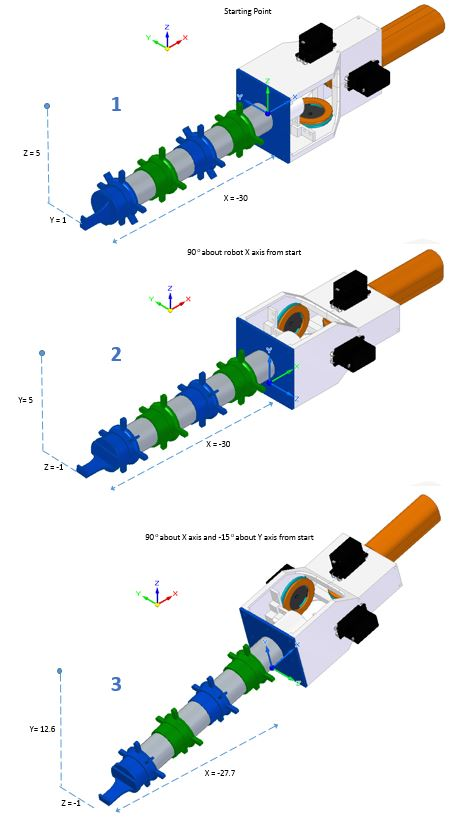
\includegraphics[width=0.6\textwidth]{images/rotationExampleAll.jpg}
\captionof{figure}{Example showing how the position and orientation of a point changes with base rotation}
\label{figure:rotationExample}
\end{center}

\begin{enumerate}
\item{The robot is in its original starting orientation, and can be said to have zero rotation about any of the axes. There is no relative difference between the axes of the robot and the global axes (shown in the top left of each image). The target point has an actual relative distance to the robot base of -30, 1 and 5 units respectively for the X, Y and Z dimensions. As there is no relative axes difference, the relative distance in relation to the robot base axes is identical in all three dimensions. As such, in this situation, the actual relative distance vector could be inserted into the regression function as is.}
\item{At the second stage, the robot has been rotated 90\degree about the global x axis. The local axis of the robot base is therefore at a relative orientation difference of the same amount. The physical relative distance of the target point to the base is unchanged, but the target point relative to the local axes of the base is different, with the local Y and Z distances being swapped around, and the latter being negated.}
\item{The final image shows the outcome if the relative rotation of the base was a 90\degree rotation about the global X axis (as in the previous image) followed by a -15\degree rotation about the global Y axis. The physical relative distance of the target point to the base is again unchanged in the global axis as the base itself has not translated in any direction. Again, the relative dimensional distances in terms of the local axes of the base are altered further, with relative values now of -27.7, 12.6 and -1 respectively for X, Y and Z. This is the vector that must be inserted into the regression function, to attain motor angles that result in a 3D point which, relative to the local axes of the base, is equal to the physical target point relative to the global and starting axes. This conversion of the target point to the local axes of the base is performed via the aforementioned steps with the negation of base angles and the rotation matrix of \ref{equation:rotationMatrix}}.
\end{enumerate}


\subsubsection{Gesturing Algorithm for Distant Targets}
In order to be cooperative and interactive in practice, a handheld robot must be able to indicate positional preferences to the user. This may entail where it must be located in order to carry out a given robotic operation, or even just the next point the user must deal with for task progression. This process is referred to as gesturing from the robot to the user towards 3D locations. In this scenario, the selected method for gesturing is comparable to typical `pointing' operations, similar to finger pointing, which is beneficial in terms of simplicity of use. Pointing is intuitive to the user as humans do this naturally to direct the attention of others to areas of interest, and is considered inherently linked to speech and communication \cite{butterworth2003}. Therefore confusion should be avoided in the user knowing where the robot desires to be relocated.

In order to gesture effectively to the user, the 3D target points must be categorised as achievable or not from the outset before deciding the next step. Initially, a point can be said to be immediately unachievable if the relative distance between itself and the base of the robot is greater than (or a certain amount less than) the typical tip-to-base distance in a straight-arm configuration. This tip-to-base distance can be used as the radius of a sphere which governs whether the points can be immediately disregarded as attainable, and requires gesturing, or whether further checking is required to assess whether it is appropriate to attempt to match this point directly. This concept is illustrated in Figure \ref{figure:tipSphere}.

\begin{center}
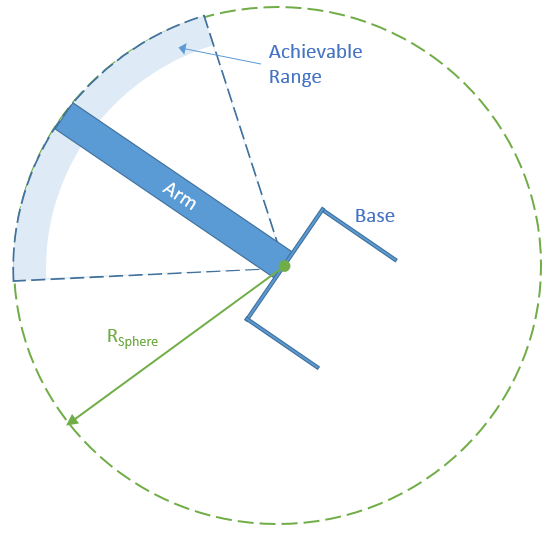
\includegraphics[width=0.6\textwidth]{images/tipSphere.png}
\captionof{figure}{Concept of tip-to-base sphere marking immediately disregarded zone, and initial achievable range zone that requires further checking}
\label{figure:tipSphere}
\end{center}

If the point lies at an absolute distance that falls within the range between the radius of the sphere and another minimum radius, $R_{minSphere}$, the point is not disregarded as being unachievable straight away. This minimum radius is determined by the smallest absolute tip-to-base difference from the stored calibration data (3D Pythagoras). However, if it lies outside this range, a new target point is required that is equivalent to shifting the original along the vector between itself and the base until it falls in this range. 

The current target then lies within this intermediate range, and there is a further check to determine whether the coordinates of the target point relative to the base fall outside any of the recorded minimum and maximum values for the X, Y and Z dimensions. If not, then the target may be directly achievable, and the positional vector is inserted straight into the regression function to check if motor angles can be yielded, giving a solution. However in the event of this still not generating a valid solution, or if the point does fall outside any of the min/max ranges, a compromise is required. This entails selecting a new target point from the stored calibration data that is geometrically closest to the target point in question. Thus, if not able to match the point, a new point should be determined to exhibit a suitable gesture motion. The typical process for responding to a far-off point is illustrated in Figure \ref{figure:gestureSolution}.

\begin{center}
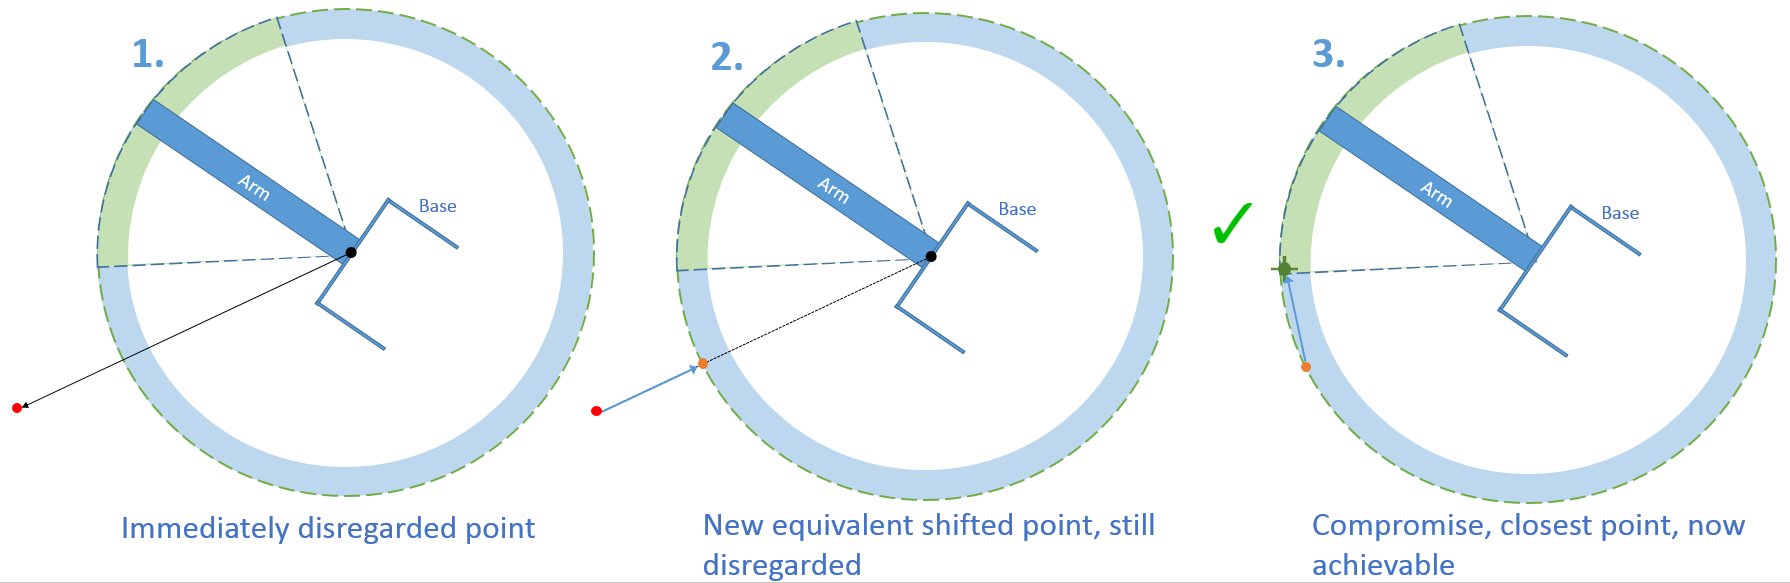
\includegraphics[width=\textwidth]{images/gestureSolution.png}
\captionof{figure}{Typical steps in obtaining a compromised gesture solution from an initially unachievable point}
\label{figure:gestureSolution}
\end{center}

\begin{enumerate}
\item{The given target point is immediately disregarded as it lies at an absolute distance above the radius of the sphere.}
\item{A new target point is formed that is the equivalent of shifting the original point along the line from itself to the base. This is done by determining the required factor to shift the target to lie on the sphere. This factor is $Shift Factor = R_{Sphere} / absolute distance$, and each coordinate of the target point is multiplied by this to give a new vector on the sphere.}
\item{The point is still unachievable as it lies beyond the max/min range of some of the dimensions from the calibration data. The compromise is therefore to find the point in the calibration data that has the closest absolute proximity to this point and use that either as an input to the function of using the stored motor angles for this point (quicker). }
\end{enumerate}


FLOW DIAGRAM OF THE TARGET POINT COMING IN, BEING CONVERTED TO CORRECT LOCAL ORIENTATION, THEN BEING CHECKED FOR BEING POSSIBLE ETC ETC BEFORE GETTING A REAL POINT AS AN INPUT

\subsubsection{Running with a Live Target in Real Time}
RUNNING THE SET MOTOR INSTRUCTION IN A DIFFERENT THREAD IN A LOOP SO TARGET CAN BE UPDATED LIVE AND THE MOTION OF THE SERVOS IS ADJUSTED LIVE SO AS TO NOT FINISH THE PREVIOUS COMMAND AND JUST CONCENTRATE ON CURRENT TARGET.

SMALL PAIR OF FLOW DIAGRAMS TO SHOW ONE THREAD CONSTANTLY UPDATING THE POSITION AND THE OTHER WORKING OUT WHAT THE POSITION SHOULD BE AND CHANGING IT BASED ON TASK PROGRESSION AND TARGET POINT ETC. THE LATTER WILL JUST SAY "POINT DETERMINATION ALGORITHM" AND WILL BE  A COMPRESSED VERSION OF THE LARGER FLOW DIAGRAM IN THE PREVIOUS SECTION.

\section{Physical Experiment}
\subsection{Setup}
\subsection{Construction Environment Parallels}
\subsection{Mental Aspect}
\subsection{Physical Aspect}

\section{Results}

\section{Discussion}
\section{Conclusion}
\section{Further Work and Areas of Improvement}

\bibliography{mybib}
\bibliographystyle{unsrt}

\section{Appendix}
\subsection{CAD Drawings}
\end{document}